\section {Числовые характеристики случайных величин: квантили. Медиана и ее свойства. Интерквартильный размах}

\begin{defn}
    \textit{Медианой} $\operatorname{Med} \xi$ распределения случайной величины $\xi$ называется любое из \textit{чисел} $\mu$ таких, что
    \begin{equation*}
        \MyPr(\xi \leqslant \mu) \geqslant \frac{1}{2}, ~~~ \MyPr(\xi \geqslant \mu) \geqslant \frac{1}{2}.
    \end{equation*}
\end{defn} 

\begin{rmrk}
    Медиана распределения всегда существует, но может быть не единственна. 
    Например, в случае дискретного распределения $\MyPr(\xi = -1) = \MyPr(\xi = 1) = \frac{1}{2}$ и $1$, и $-1$ удовлетворяют определению медианы.
\end{rmrk} 

\begin{defn}
\textit{Квантиль порядка $\gamma$}~--- это такое число $\kappa_\gamma$, для которого выполняется
\begin{equation*}
    \begin{cases} 
        \MyPr(\xi \leqslant \kappa_\gamma) = F(\kappa_\gamma) \geqslant \gamma, \\
        \MyPr(\xi \geqslant \kappa_\gamma) = 1 - F(\kappa_\gamma + 0) \geqslant 1 - \gamma 
    \end{cases}
\end{equation*}
\end{defn}

\begin{rmrk}
    Если функция распределения $F$ непрерывна и строго монотонна, то \textit{квантилем} порядка (уровня) $\gamma$, где $\gamma \in (0; 1), $ является решение $x_\gamma$ уравнения $F(x_\gamma) = \gamma.$ 
    Тогда квантиль порядка $\gamma$ отрезает от области под графиком плотности область с площадью $\gamma$ слева от себя. Справа от $\kappa_\gamma$ площадь области равна $1 - \gamma$.
    
    Если же случайная величина не является абсолютно непрерывной, то уравнение $F(x_\gamma) = \gamma$ может не иметь решений. Например, для приведенного ниже графика не существует $x_{\frac{1}{2}}: F(x_{\frac{1}{2}}) = \frac{1}{2}$.
    %sec1-6
\begin{center}
    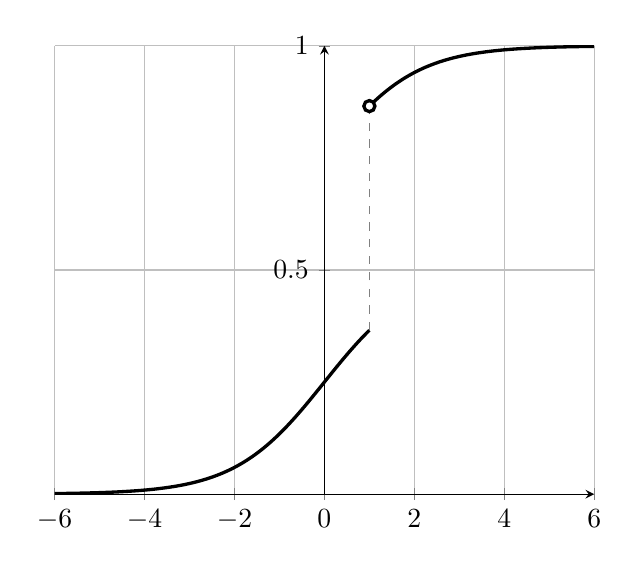
\begin{tikzpicture}[
        declare function={
            sigma(\x)=1 / (1 + exp(-\x));
            F(\x) = .5 * sigma(\x);
        }]
        \begin{axis}[
            grid=major,     
            xmin=-6, xmax=6,
            ymin=0, ymax=1,
            ytick={0,.5,1},
            axis x line=bottom,
            axis y line=middle,
            samples=100,
            legend style={at={(1,0.9)}}     
        ]
        \addplot[very thick,black,mark=none, domain=-6:1]   {F(x)};
        \addplot[very thick,black,mark=*,mark options={fill=white},domain=1:6, mark repeat=1000]    {F(x)+0.5};
        \draw [dashed,black!50] (1,{F(1)}) -- (1,{F(1)+0.5});        
        \end{axis}
    \end{tikzpicture}
\end{center}
\end{rmrk} 

\begin{defn}
    Квантили уровней, кратных $0.01$, называют \textit{процентилями}, квантили уровней, кратных $0.1$, — \textit{децилями}, уровней, кратных $0.25$, — \textit{квартилями}.
\end{defn} 

\begin{rmrk}
    Медиана является квантилем уровня $1 / 2$.
\end{rmrk} 

\begin{namedthm}[Свойства медианы]\leavevmode
\begin{enumerate}
    \item Медиана случайной величины $\xi$ минимизирует средний модуль отклонения $\xi$:
    \begin{equation*}
        \Exp |\xi - \operatorname{Med} \xi| 
    = \min _{a} \Exp |\xi-a|;
    \end{equation*}
    \item Отклонение медианы случайной величины $\xi$ от её матожидания $\Exp \xi$ не превышает по модулю среднеквадратичного отклонения $\sigma = \sqrt{\Var\xi}$:
    \begin{equation*}
        |\Exp \xi - \operatorname{Med}\xi| \leqslant \sigma.
    \end{equation*}
\end{enumerate}
\end{namedthm}

\begin{proof}
    \begin{enumerate}
        \item Рассмотрим случайную величину $\eta = \xi - \operatorname{Med}\xi$. 
        Очевидно, что $\operatorname{Med} \eta = 0$. 
        Тогда нам надо показать, что $\forall c \in \Real $ справедливо 
        \begin{equation*}
            \Exp |\eta - c| - \Exp |\eta| \geqslant 0.
        \end{equation*}
        
        Рассмотрим случай $c > 0$. Заметим, что 
        \begin{equation*}
            \begin{cases}
                |\eta - c| - |\eta| = c, & \eta < 0; \\
                |\eta - c| - |\eta|  \geqslant -c, & \eta \geqslant 0.
        \end{cases}
        \end{equation*}
        
        Тогда
        \begin{gather*}
            \Exp \bigl(|\eta - c| - |\eta| \bigl) 
            = \Exp \bigl( (|\eta - c| - |\eta|) \cdot \Ind(\eta < 0) + (|\eta - c| - |\eta|) \cdot \Ind(\eta \geqslant 0) \bigl) \\
            \Exp \bigl( |\eta - c| - |\eta| \bigl) \geqslant c~\MyPr(\eta < 0) - c~\MyPr(\eta \geqslant 0).
        \end{gather*}
        Так как $\operatorname{Med}\eta = 0$, то $\MyPr(\eta \leqslant 0) = \MyPr(\eta \geqslant 0) = \frac{1}{2} \implies \Exp \bigl( |\eta - c| - |\eta| \bigl) \geqslant 0.$.

        Случай $c < 0$ сводится к предыдущему умножением случайной величины и $c$ на $-1$. Отсюда следует, что медиана действительно минимизирует средний модуль отклонения.

        \item Рассмотрим цепочку неравенств:
        \begin{multline*}
            |\Exp \xi - \operatorname{Med}\xi| =
            |\Exp (\operatorname{Med}\xi - \xi)| \leqslant
            {\text{\{св-во (6) матожидания\}}} \leqslant 
            \Exp |\operatorname{Med}\xi - \xi| \leqslant \\ {\text{\{св-во (1) медианы\}}} \leqslant
            \Exp | \Exp \xi - \xi| = 
            \Exp \sqrt{|\Exp \xi - \xi|^2} \leqslant
            {\text{\{нер-во Йенсена\}}} \leqslant \\
            \leqslant \sqrt{\Exp | \Exp \xi - \xi|^2} = \sqrt{\Var\xi} = \sigma.
        \end{multline*}
        
    \end{enumerate}
\end{proof}
\begin{defn}
    \textit{Интерквартильным размахом} называется разность между третьим и первым квартилями, то есть ${\displaystyle x_{0{,}75}-x_{0{,}25}}.$
\end{defn} 

В каком-то смысле эту величину можно считать аналогом дисперсии случайной величины, устойчивой к выбросам.
